\begin{chapter}{Heteroscedastic \& Multilevel GP Emulators For Stochastic Simulators\label{Ch:Hetsml}}


The majority of this chapter is based upon \citet{Kennedy2020}.
\section{Introduction}
The previous chapter of this thesis focused on using GP priors to model complex computer simulators. We reviewed many of the more classical emulation strategies which were mostly developed between the $1980$'s and early $2000$'s. This literature focused on \textit{deterministic} simulators, since, at the time, they were probably the most common type of simulation model \citep{Sacks89,Craig1997, Ohagan01, Santner2003}. These deterministic models were implemented even if the corresponding real world process exhibited stochasticity \citep{Ohagan01}. Of course, this absent stochasticity `wrong', as are all models. Nonetheless, these deterministic models still have practical value\georgebox.

To incorporate uncertainty into predictions, modellers have produced increasing numbers of stochastic simulators. As stochastic simulation has become more prominent across all sciences, so has the interest in the emulation of stochastic computer simulators \citep{Astfalck19, Rocchetta2018, Boys2018}. There are a variety of approaches to (GP based) emulation of stochastic computer models; see \citet{Baker2022} for a recent overview.

The simplest approach to modelling stochastic simulators, which was outline in the previous chapter, is to add $\lambda^2 I$ to the covariance structure. This approach is rather limiting when $\var\{ y(\bx) \}$ is thought to depend on $\bx$. A canonical example of heteroscedasticity is the motorcycle data set, which comes directly from a stochastic computer experiment. Although \citet{Silverman1985} fit splines to this data, we will continue to use GPs and start with a homoscedastic GP (HomGP).
\begin{figure}[ht]
	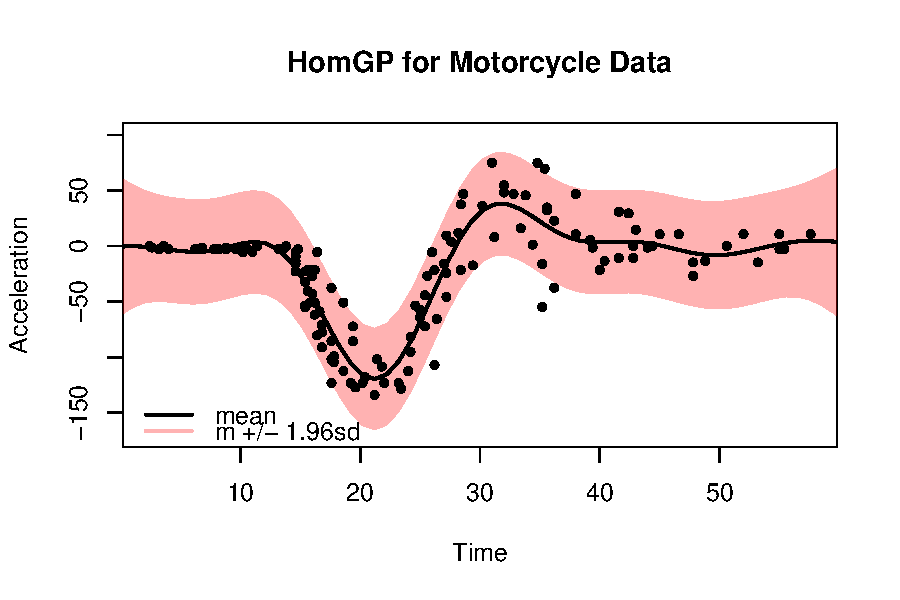
\includegraphics{fig-het-sml/mcycle-homgp.pdf}
	\caption{The motorcycle data set with a HomGP superimposed. The black line is the emulator mean and the red band corresponds to a $95\%$ posterior predictive interval for $y(x)$.}
	\label{Fig:mcycle-hom}
\end{figure}
Observing the fitted mean function in \Cref{Fig:mcycle-hom} for the motorcycle data is reasonable. The pitfall is the emulator's predictive variance is a poor match for the variability in the data, thus interval estimates for $y(\bx)$ are poorly calibrated. There will also be a knock-on effect on uncertainty quantification about $\E \{ y(\bx) \}$. The misspecified variance is most prominent for $\text{Time}<15$ where it is clear that $\var \{y(\bx) \} \approx 0$ but the emulator estimates $\var\{ y(\bx) \mid \mathcal{D}) \approx 28$. The variance also looks too large for $\text{Time}>40$. The predictive variance is reasonably accurate for $\text{Time} \in [15, 40]$. Ultimately to produce a good surrogate for heteroscedastic simulators, we need to produce emulators with a heteroscedastic element baked into them. Our goal here is to find approaches that
\begin{itemize}
	\item[(i)] produce a mean estimate of $y(\bx)$;
	\item[(ii)] quantify uncertainty in $\E \{ y(\bx) \} $;
	\item[(iii)] provide flexible estimates of $\lambda^2(\bx) = \var\{ y(\bx) \}$.
\end{itemize}

\section{Separate Mean and Variance Emulation}

To estimate the mean response of a heteroscedastic stochastic simulator, we might apply Stochastic Kriging (SK) to runs of the simulator \citep{Akenman2010}. SK is similar to the constant noise set up. The difference being that instead of having a (prior) covariance matrix of the form $\var\{y (X)\} = C(X, X) + \lambda^2 I$, we have
\begin{equation}
	\var\{y (X)\} = C(X, X) + \diag\left( \frac{s^2(\bx_1)}{r_1},\frac{s^2(\bx_2)}{r_2}, \ldots, \frac{s^2(\bx_k)}{r_k} \right)
\end{equation}
as the covariance matrix, where $s^2(\bx_i)$ is the (sample) variance based on $r_i$ replicated runs of $y(\bx_i)$. For SK it is recommend that $r_i \geq 10$. This deals with the heteroscedasticity at the design points since the nugget term depends on $\bx$. However, the noise is treated as a nuisance rather than as part of the problem; SK only emulates $\E \{ y(\bx) \}$. Emulating stochastic computer models can be viewed as modelling a multiple output simulator. If both outputs (mean and variance) are important, then we need to explicitly model $\lambda^2(\bx)$.

\citet{Henderson09} construct two independent GP emulators. One for $\E \{y(\bx) \}$ and another for $ \log \lambda(\bx)$. Note that \citet{Henderson09} emulate the log standard deviation, rather than log variance, but these are identical up to a multiplicative factor of $2$. Their case study employs around $1000$ replicates per design point; this does not take too long for their example (they generate their training data in about a day using parallel computing) but for more expensive simulators this may be an unachievable sample size. Simple sample mean and standard deviation estimates to construct their emulators. This independence assumption is pragmatic; the simulator mean and standard deviations are both functions of $\bx$, but it is a practical and useful modelling choice\georgebox. This pragmatic approach is also adopted by \citet{Andrianakis2017} and is shown to be more powerful than taking $\lambda^2(\bx) = \lambda^2$.

\citet{Marrel2012} take a similar approach to \citet{Henderson09} but couple together their mean variance GPs. They first estimate the mean response using a HomGP, let the posterior mean be $m_0(\bx)$. Next they estimate $\var\{ y(\bx) \} \approx \frac{1}{r} \sum_{i=1}^r (y_i(\bx) - m_0(\bx))^2$ and fit a GP to estimated variances, let the posterior mean of this GP be $m_V(\cdot)$. They then fit a new GP to $y(\bx)$ using $m_V(\cdot)$ in place of $\lambda^2$: $y(\cdot) \sim \mathcal{GP} \{ m(\cdot), C(\cdot, \cdot) + m_V(\cdot)I \}$. The authors suggests that this approach may be improved my alternating between fitted the variance GP and the mean GP until some convergence criterion is met.

\subsection{Non-Normal Noise}
If the stochasticity exhibited by $y(\bx)$ is not close to a Normal distribution (e.g. asymmetric), then more work may have to be done. Transformation is a For example, if it is known that $y(\bx) > 0$ a log transform may be enough to rectify non-Normality. The availability, $A(\bx)$, in Athena is constrained to the unit interval thus constructing an emulator for $\logit A(\bx)$ or $\probit A(\bx)$ would be a sensible strategy.

If the simulator behaviour is too complex to be made (approximately) Gaussian by transformation, Quantile Kriging may be an appropriate tool \citep{Plumlee2014}. Since quantiles are directly estimated, rather than moments, Quantile Kriging is highly flexible and can reproduce complex simulator behaviour such as multimodal outputs and discrete outputs without any additional modelling. This is perhaps the most flexible approach to modelling stochastic simulators. This flexibility comes at a large cost; hundreds of replicates are required to model non-Gaussian, input dependent, noise in computer simulators. Many stochastic simulators, such as Athena, can be computationally expensive. Thus such levels of replication could make emulation of the Athena, and other simulators, infeasible unless huge computing budgets are available.

Another approach to using GPs to model simulators which are asymmetric or otherwise non-Normal is to embed a GP into another statistical model. This is an attractive approach since it may help leverage problem structure. For example, if a model outputs an integer (perhaps, the number of cells that have mutated in a biological system), we may wish to model the response as $y(\bx) \sim \text{Poisson}\,(\gamma(\bx))$ with $\log \gamma (\cdot) \sim \mathcal{GP} \{m(\cdot), C(\cdot, \cdot) \}$. Note the lack of nugget term in the GP because the stochasticity is absorbed into the Poisson error structure (and other non-Gaussian models which utilise a GP). A Bayesian treatment would require intensive numerical methods to integrate out the latent GP to form the posterior density for $y(\bx)$ in this Poisson model. For this reason, the person constructing may prefer to employ the tractable and computationally efficient GP over a more accurate, but unwieldy non-Gaussian emulator. For example, the capture-recapture example illustrated in \citet{Baker2022} is non-Gaussian but the (computational) advantages of employing a GP surrogate outweigh this misrepresentation of the simulator\georgebox.

If the response is non-Gaussian but all that is required is a central estimate and quantification of uncertainty a Bayes Linear approach may be useful. If probabilistic predictions are required, the adjusted moments can be plugged into a parametric form. For example, \citet{Jackson2019} use a Bayes Linear emulator to find the adjusted mean and variance of a simulator, then plug these moments into (i) a Normal distribution and (ii) a uniform distribution to construct probabilistic predictions for a deterministic simulator. This approach of plugging moments into a parametric form can easily be adapted to stochastic simulations. However, those utilising a Bayes Linear approach prefer not to assume any probabilistic form and report only the adjusted moments.

\section{Heteroscedastic Gaussian Processes}

The approaches mentioned so far in this chapter typically rely on using multiple emulators to generate prediction for a single quantity of interest; $y(\bx)$. There is something dissatisfying about requiring two independent, statistical models to make predictive statements about a single quantity of interest. A unified approach is appealing.

Unification of mean and variance emulators motivates the Heteroscedastic Gaussian Process (HetGP), which originated in the machine learning literature as a regression procedure \citep{Goldberg1998} but has recently gained traction in the emulation literature for modelling simulators exhibiting input dependent noise \citep{Binois2018, Baker2020c}.

\subsection{The HetGP Emulator}

If $y(\cdot)$ is a stochastic computer model, then the HetGP emulator is as follows:
\begin{align}
y(\cdot) | \lambda^2(\cdot) &\sim  \mathcal{GP} \{ \mu(\cdot), C(\cdot, \cdot) + \lambda^2(\cdot) \} \label{Eq:} \\
\log \lambda^2 (\cdot) &\sim  \mathcal{GP} \{ \mu_V (\cdot), C_V (\cdot, \cdot) + \lambda_{V}^2 I \}.
\end{align}
An alternative representation is $y(\cdot) = f(\cdot) + \sqrt{\lambda^2(\cdot)} \varepsilon$  where $f(\cdot) \sim \mathcal{GP}\{ \mu(\cdot), C(\cdot, \cdot) \}$, $\log \lambda^2(\cdot) \sim \mathcal{GP}\{\mu_V(\cdot), C_V(\cdot, \cdot) + \lambda_V^2I \}$ and $\varepsilon \sim N(0, 1)$.

Here, $\mu(\cdot)$ and $C(\cdot, \cdot)$ are mean and covariance functions (respectively) for $f(\cdot) = \E \{y(\cdot)\}$. $\mu_V(\cdot)$ and $C_V(\cdot, \cdot)$ are the mean and covariance functions for $\E\{ \log \lambda^2(\cdot) \}  $ and $\lambda_V^2 I$ denotes a constant nugget effect for the log variance. Now $\var(y(\bx)) = C(\bx, \bx) + \lambda^2(\bx)I$ depends explicitly on $\bx$ even if $C(\cdot, \cdot)$ is a stationary covariance function, thus HetGP is a type of non-stationary GP. \citet{Boukouvalas2010} proposed simplifying the HetGP by replacing the GP prior on $\log \lambda^2 (\cdot)$ by a known parametric form with parameters to be inferred.

A unique selling point of the HetGP is that it need not require replication, but still allows for it. The allure of HetGP is the promise of a full surrogate; joint prediction of the mean response and the level of noise at any input combination. This is possible via a latent variable formulation which jointly models the simulator mean as a GP and the log noise (to ensure positivity) as a GP. As \citet{Gramacy2020surrogates} notes, this coupled GP approach provides smooth estimates of the noise at both within sample and out of sample simulator inputs.

As with the previous chapter, we will assume squared exponential covariance functions for $C(\cdot, \cdot)$ and $C_V(\cdot, \cdot)$, but this is not a requirement. The \texttt{hetGP} package allows for other covariance functions such as Mat\'ern \cite{hetGP}. Parameters for the simulator mean, $f(\cdot)$, will be the same as in the previous chapter. The equivalent parameters for $\log \lambda^2 (\cdot)$ will have a $V$ subscript. To our knowledge, no previous work on using HetGPs considers parameter uncertainty in a tractable format; \citet{Goldberg1998} consider some suitable MCMC scheme for full Bayesian computation. We will take a slight diversion now to outline our partially Bayesian HetGP, which does not require intensive computation for inference or prediction.

\subsection{A Bayesian HetGP}

Our approach to a tractable, but Bayesian, HetGP is to integrate out the $\beta$ parameters of all regression components in the two GPs. First consider the latent log-variance GP:
\begin{equation}
	\log \lambda^2(\cdot) \mid \Theta_V \lambda_V \sim \mathcal{GP} \{ h_V(\cdot)^T \beta_V , C_V(\cdot, \cdot) + \lambda^2_V I\}
\end{equation}
where $\Theta_V$ are the hyperparameters of $C_V(\cdot, \cdot)$. Since the above is just a homoscedastic GP, if we place the prior $\beta_V \sim \mathcal{N}\{\bm{b}_V, B_V \}$ then using standard properties of Normal RVs we arrive at
\begin{equation}
	\log \lambda^2(X) \mid \sigma_V, \theta_V, \lambda_V \sim \mathcal{GP} \{ H_V \bm{b}_V , C_V(X, X) + H_V B_V H_V^T + \lambda^2_V I\}
\end{equation}
where the $i$-th row of $H_V$ corresponds to $h_V(\bx_i)$. As with the GPs presented in \cref{Ch:Emulators} we will use the notation $K(\cdot, \cdot)$ to represent a covariance function after integrating out regression coefficients. A $V$ subscript is used when referring to aspects of $\log \lambda^2 (\cdot)$. The posterior moments of $\log \lambda^2(\cdot) \mid \Theta_V$ are a direct consequence of the multivariate Normal equations;
\begin{align}
	\log \lambda^2(X^*) \mid \Theta_V, \log \lambda^2(X) &\sim \mathcal{N} \{ m^*_V(X^*), v_V^*(X) \} \label{Eq:bayes-post-lambda} \\
	m_V^*(X^*) &= H^* \bm{b}_V - K_V(X^*, X) K_V(X, X)^{-1} (\log \lambda^2(X) - H_V \bm{b}_V)\\
	v_V^*(X^*) &= K(X^*, X^*) - K_V(X^*, X) K_V(X, X)^{-1} K_V(X, X^*) + \lambda^2_V I
\end{align}
Then our model for the observable $y(\bx)$ is
\begin{equation}
	y(\cdot) \mid \beta, \Theta, \lambda^2(\cdot) \sim \mathcal{GP} \{ h(\cdot)^T \beta, C(\cdot, \cdot) + \lambda^2(\cdot)I \}.
\end{equation}
where $\Theta$ denotes $\Theta_V$ and all the hyperparameters of $C(\cdot, \cdot)$, namely $\Theta = \{\Theta_V, \sigma, \theta_1, \theta_2, \ldots, \theta_k \}$. Now we can integrate out $\beta \sim \mathcal{N}(\bm{b}, B)$ in the usual way leading to
\begin{equation}
	y(X) \mid \Theta, \lambda^2(\cdot) \sim \mathcal{N} \{ H\bm{b}, K(X, X) + \lambda^2(X)I \}
\end{equation}
where $K(X, X) = HBH^T + C(X, X)$ is the covariance function of $\E \{y(X))\}$ after integrating out $\beta$. Under this approach, we need to obtain a point estimate of $\lambda^2(\bx)$ from \cref{Eq:bayes-post-lambda}. Obvious candidates are the posterior mean, median and mode of $\lambda^2(X^*)$. Since $\log \lambda^2(X)$ is Normal, $\lambda^2(X)$ is log Normal and thus:
\begin{align}
	\E \{\lambda^2(X^*) \mid \mathcal{D}, \Theta \}  &= \exp \{ m_V^*(X^*) + \frac{1}{2}v_V^*(X^*) \}\\
	\text{mode}\, \{\lambda^2(X^*) \mid \mathcal{D}, \Theta \} &= \exp \{ m_V^*(X^*) - v_V^*(X^*) \}\\
	\text{median}\, \{\lambda^2(X^*) \mid \mathcal{D}, \Theta \} &= \exp \{ m_V^*(X^*)\}.
\end{align}
 The most conservative estimate is the mean, whereas the mode will be the most optimistic. All three will be approximately equal when $|v_V^*(X^*)|<<|m^*_V(\bx)|$. Thus, if this is thought to be the case, we would recommend using the median point estimate as this doesn't rely on $v_V^*(X^*)$ and thus is fastest to compute. The speed difference will be greatest for larger sample sizes, and typically $v_V^*(X^*)$ will be small for large sample sizes. Also small $\sigma_V$ and $\lambda_V$ lead to small $v_V^*(X^*)$.
\subsection{Back to Motorcycles}

Returning to the motorcycle example, \Cref{Fig:mcycle-het}, presents a HetGP fitted to the motorcycle data. The predictive intervals provided by the HetGP emulator are much more appropriate than those from the HomGP emulators. The interval width starts off small, is wider in the region of $15 < \text{Time} < 30$ then shrinks again for $\text{Time} > 30$, mimicking the input-dependent variability in the data.
\begin{figure}[ht]
	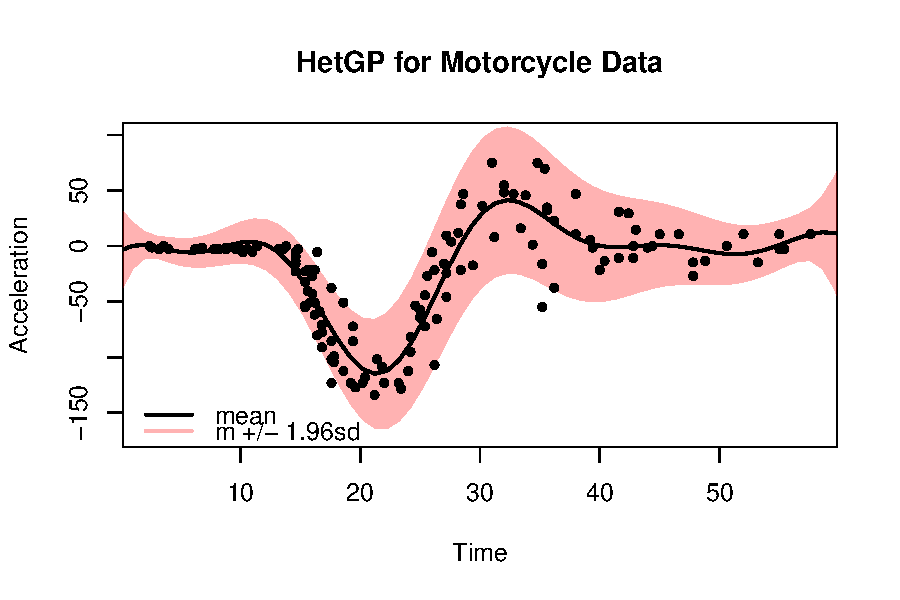
\includegraphics{fig-het-sml/mcycle-hetgp.pdf}
	\caption{The motorcycle data set with a HetGP superimposed. The black line is the emulator mean and the red band corresponds to a $95\%$ posterior predictive interval for $y(x)$.}
	\label{Fig:mcycle-het}
\end{figure}
Hopefully \cref{Fig:mcycle-het} convinces the reader that HetGPs are great at detecting non-linear variability in both the mean response surface of a simulator and also the mean. However, this model is incredibly data-hungry;  \citet{Binois2018, Zhang2020} both used hundreds of runs per input dimension; the single input motorcycle example has a sample size of $133$.
\subsection{Shortcomings of HetGP \label{hetgp-shortcomings}}

We often construct emulators because the data (simulator runs) are scarce. Let us consider a simple, tractable and heteroscedastic stochastic simulator, defined for $x \in [0,1]$:
\begin{align}
	y(x) &= 4\sin(7 \pi x) + 5(2x + 1) + 3 \log (x + 0.01) + (5x + 2)\varepsilon\label{Eq:toy-stoch}\\
	\varepsilon &\iid \mathcal{N}(0,1).
\end{align}
This simulator is incredibly simple and virtually instantaneous to run, thus is used only for illustrative purposes.
\begin{figure}[ht]
	\centering
	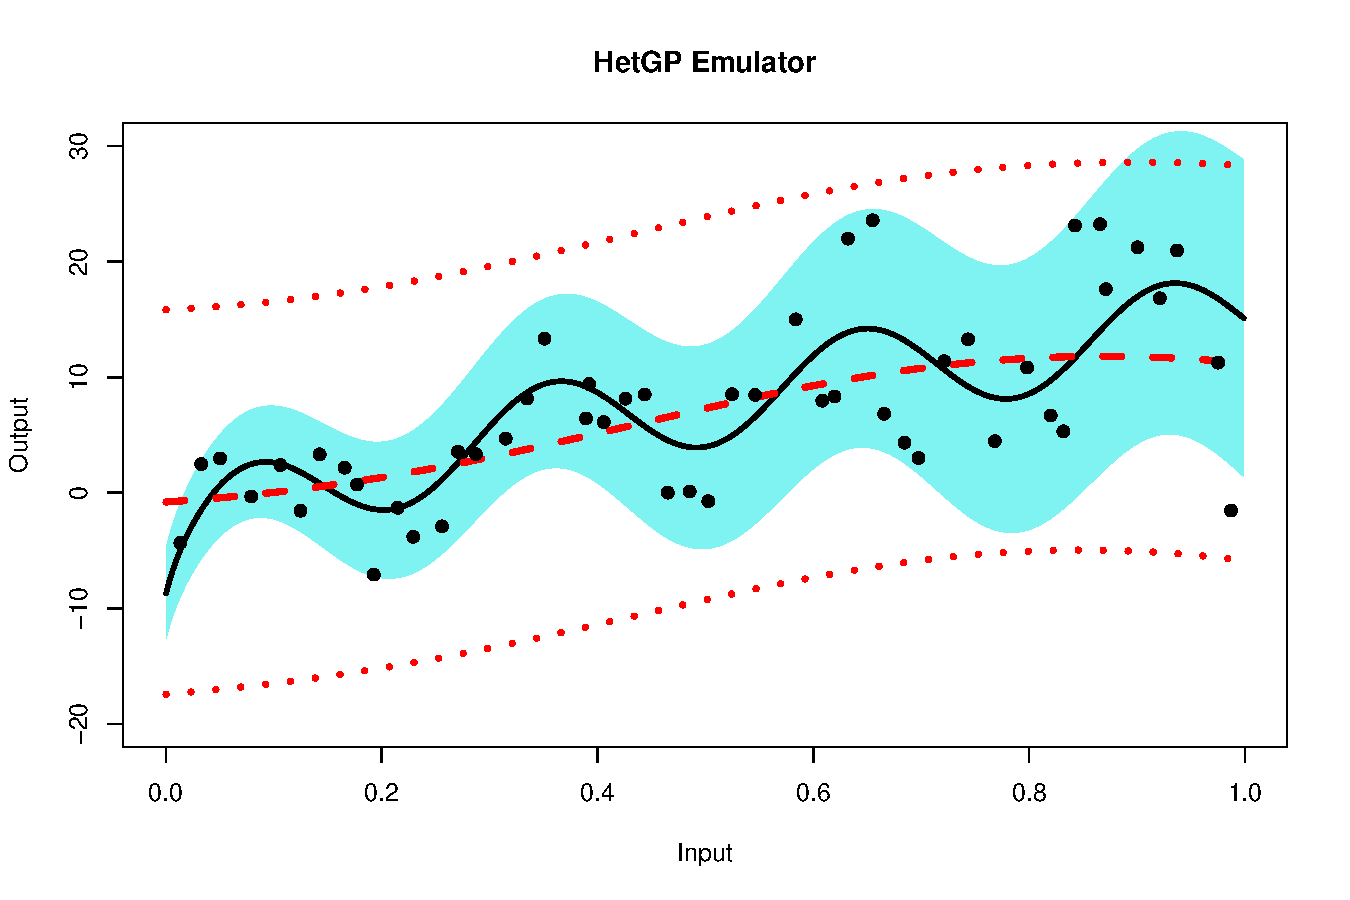
\includegraphics[width=0.75\textwidth]{sml-het-fig2/toy-hgp.pdf}
	\caption{A HetGP emulator for \Cref{Eq:toy-stoch}. Black points are the outputs from $50$ runs of the simulator. Black line represents the true simulator mean and the blue band represents the mean $\pm 1.96$ `true' standard deviations. Red dashed line represents emulator mean with red dotted lines being the emulator mean $\pm 1.96$ emulator standard deviations.}
	\label{Fig:toy-HetGP}
\end{figure}
Observing the fit in \Cref{Fig:toy-HetGP}, the fitted emulator mean (dashed red line) does not match up well with the simulator. The emulator predicts an approximately linear response whereas the simulator is clearly sinusoidal in nature. The emulator is interpreting the systematic sinusoidal variation as noise, rather than signal. Ultimately, this is because emulating a stochastic computer model requires much more information than the standard deterministic problem. However, when provided with adequate amounts of data, HetGP can produce excellent surrogates for complex stochastic computer models \citep{Binois2018}. The emulator in \label{Fig:toy-HetGP} has interpreted the systematic, sinusoidal, variation as noise rather than signal. This is a similar phenomenon to that observed by \citet{Andrianakis2012}, they observed that $(\lambda, \theta)$ often have a bimodal likelihood when emulating deterministic simulators, with one mode corresponding to large $\lambda$. In other words, it is not uncommon for the emulator to favour an overly smooth fit. There are essentially three ways in which a HetGP can interpret variability in a stochastic simulation:
\begin{itemize}
	\item[(1)] Low signal; high noise. In this case $\lambda^2(\cdot)$ is over-estimated, resulting in an overly-smooth mean response. This is what has happened in \Cref{Fig:toy-HetGP}.
	\item[(2)] Low noise; high signal. This is where $\lambda^2(\cdot) \to 0$ and then the mean function interpolates the data as if the simulator were deterministic.
	\item[(3)] A Goldilocks fit, i.e somewhere in between the other two. In this case, the HetGP will manage to tease the noise from the signal and produce an appropriate fit akin to \Cref{Fig:mcycle-het}.
\end{itemize}
When simulator runs are sparse, it is quite easy to end up in scenario (1). In our experience, (2) is very rare, but is still possible. To end up in (3), the ideal scenario, we need to either have a (relatively) large number of simulator runs to allow HetGP to detect signal or some strong (and fairly accurate) beliefs about $y(\cdot)$ expressed via $\mu(\cdot)$  and $C(\cdot, \cdot)$. However, if $y(\cdot)$ is a complicated simulator which implements cutting-edge science, there may be limited knowledge of appropriate choices for $\mu(\cdot)$  and $C(\cdot, \cdot)$. It is commonly the case that we are emulating $y(\cdot)$ to perform inference about $\mu(\cdot)$.

\section{Stochastic multilevel emulation}
\label{sec:SML}
On many occasions, HetGPs require a lot of information to produce an adequate approximation to the simulator under study. To satisfy the appetite of HetGP we can provide HetGP with runs from a related, but cheaper, version of the simulator under study. This motivates the stochastic multilevel (SML) emulator proposed by \citet{Kennedy2020}, which we will discuss, implement and compare to HetGP. We also compare two estimation routines for the HetGP and SML emulators.

\subsection{Motivation and intuition}

In the Athena simulator it is simple to change model features to give us cheap approximations to large offshore wind farm simulations. Since these approximations are relatively computationally cheap, it is easy to get enough training data to construct good emulators. If we can build a good emulator for the cheap simulator, and accurately describe its mean, perhaps we can utilise this information to build better emulators for more expensive stochastic computer models.

Exploiting cheap approximations to an expensive simulator has been tackled in the deterministic framework by \citet{Kennedy2000}. The most popular format is their autoregressive structure for functions \citep{Forrester2007, Singh2017, Harvey2018}. The autoregressive structure builds a well informed emulator for the cheap simulator and uses this as a ``starting point'' for the expensive simulator. The main aim of multilevel emulation is an improved emulation of the simulator at a fixed training budget. We extend this to the more complex case of stochastic computer experiments to enhance the emulation of the Athena simulator.


In this section, we outline our proposed approach to stochastic multilevel (SML) emulation of stochastic simulators. This naturally extends deterministic emulation techniques and exploits the cheap approximations that are readily available from the Athena simulator. This approach is quite general and will apply to many stochastic simulators when cheap approximations are available. Many stochastic computer simulators have a complexity parameter, such as the length of a time step, or granularity of a grid over space, which exchanges simulation accuracy for computational cost; examples include \cite{Kennedy2000} and \citet{Le2014}. In our wind farm setting this will be the time step, $\Delta t$, in a numerical integration within each simulation run.

 The number of event times is affected by $\Delta t$, which generates the random time between events. Accurate runs ($\Delta t = 0.001$) of the Athena simulator take just over $3$ minutes for a wind farm with $200$ turbines on a desktop PC with $8 \times 3.20 \,\text{GHz}$ processors and $16\,\text{GB}$ RAM. On the same machine, cheap runs ($\Delta t = 0.1$) take just under $3$ seconds. A single expensive run is computationally equivalent to $60$ cheap runs. The accuracy required comes at a computational cost which severely hinders the size of our computer experiment, limiting the quality of the fitted emulator. We aim to exploit these computational properties in jointly modelling the ``cheap'' simulator and ``expensive'' simulator. The outputs from cheap and expensive versions of stochastic simulators will be related. Runs from both versions are combined to build an overall better emulator.

 The two levels of the Athena simulator are approximately linearly related; see \Cref{Fig:cheapandexp}. The relationship is not exact, partially due to the stochasticity of the two levels. The relationship flattens off when the probit cheap code exhibits values above about $1.6$.
\begin{figure}[ht]
  \centering
  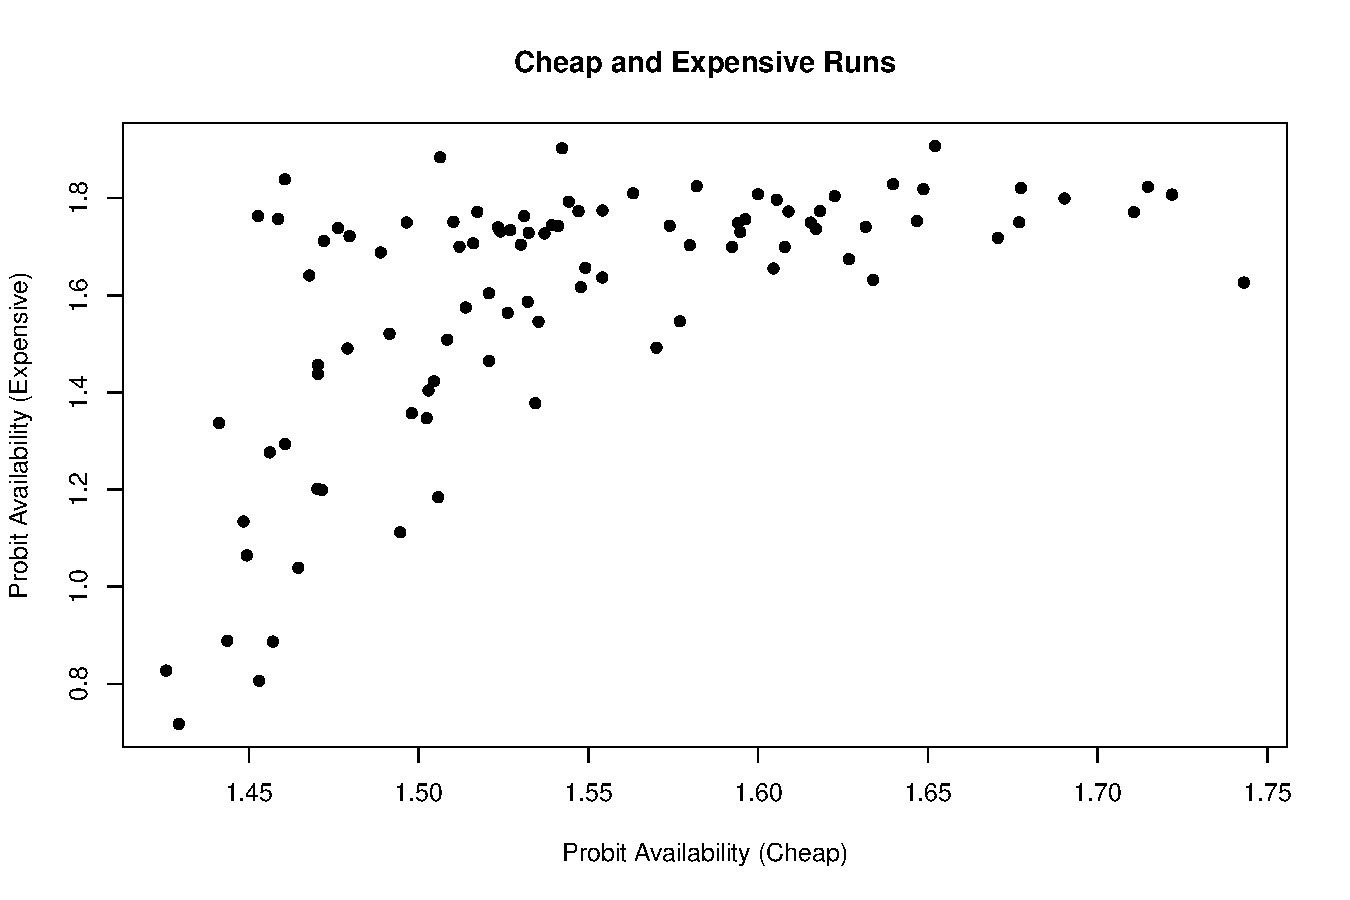
\includegraphics[width=0.75\textwidth]{sml-het-fig2/cheapVexp.pdf}
\caption{Mean probit availability under the cheap version plotted against the expensive version. Each point is computed via $10$ replications. We see an approximately linear relationship between the two levels of code but note that the range of the axes is quite different: $0.7<\text{Expensive}<2$ but $1.4<\text{Cheap}<1.8$. }
  \label{Fig:cheapandexp}
\end{figure}
We will focus on a two level set up;  $y^C(\cdot)$ is the cheap simulator and $y^E(\cdot)$ is its expensive counterpart. In the motivating example of the Athena simulator $y^C(\cdot)$ is a version of the model with a time step of $\Delta t = 0.1$ years ($\approx 1$ month. We want to infer $y^E (\cdot)$, which is a version with time step $\Delta t = 0.001$ years ($approx 9$ hours).
\subsection{Proposed emulation strategy}
We allow for $y^E(\cdot)$ to be heteroscedastic but if we believe it is homoscedastic we can replace the non-constant variance with a constant term. Our object of inference is (the distribution of) $y^E(\bx)$, for any $\bx$.

Suppose that the cheap simulator, $y^C(\cdot)$ can be modelled by a homoscedastic (constant noise) GP with mean function $m_C(\cdot)$, covariance function $C_C(\cdot, \cdot)$ and constant variance $\lambda^2_C$, that is,
\begin{equation}
	y^C(\cdot) \sim \mathcal{GP} \left( m_C(\cdot), C_C(\cdot, \cdot) + \lambda^2_C  I\right).
\end{equation}
We expect that the cheaper simulator's mean is informative for the expensive counterpart and thus, as in \cite{Kennedy2000}, we assume that
\begin{equation}
	y^E(\cdot)|\rho, \E\{y^C(\cdot)\}, \delta(\cdot) = \rho \E\{ y^C(\cdot) \} + \delta(\cdot)
\end{equation}
where $y^E (\cdot)$ is the expensive stochastic simulator and $\delta(\cdot)$ is a HetGP such that
\begin{align}
	\delta(\cdot)|\lambda_E^2 (\cdot) \sim \mathcal{GP}\left( m_E(\cdot), C_E(\cdot, \cdot) + \lambda^2_E(\cdot)I \right) \\
\log \lambda^2_E(\cdot) \sim \mathcal{GP} \left( m_V(\cdot), C_V (\cdot, \cdot) + \lambda_{V}^2 I \right),
\end{align}
where the $I$ are identity matrices of appropriate dimensions.
In this formulation, $\rho \in \R$ is a regression parameter and $m_E(\cdot)$, $C_E(\cdot, \cdot)$ are mean and covariance functions for $\delta(\cdot)$. The term $\delta(\cdot)$ serves a dual purpose. Firstly, $\delta(\cdot)$ can be viewed as a discrepancy function; the mean of $\delta(\cdot)$ represents the difference in the mean response of the two simulators, or the loss of accuracy from running cheap simulations (with a large time step/coarse grid). Secondly, $\delta(\cdot)$ describes the stochasticity in the expensive simulator. This is a similar structure to that of Bayesian calibration of deterministic computer models \citep{Ohagan01}, however we do not observe data from a physical system --- but a computer simulator --- and we have noise in both sets of observations.

This joint model for the two simulators allows us to borrow information from the cheaper simulator, but is sufficiently flexible to reject a relationship between the two levels if no such relationship exists. If $\rho = 0$ we recover HetGP.

We express the mean functions in a hierarchical form so that	$m_C(\bx) = h(\bx)^T \bm{\beta}_C$ and $m_E(\bx) = h(\bx)^T \bm{\beta}_E$. We take $h(\cdot)$ to be a set of known, deterministic basis functions. The mean functions have the same form; the particular parameters of these regression functions are allowed to differ.

We will use squared exponential covariance functions so that
\begin{equation*}
  C_{*}(\bx, \bx') =  \sigma^2_{*} \exp\left\{ -(\bx - \bx')^T D^{-1}_{*}(\bx -  \bx')\right\}
\end{equation*}
where $* \in \{C, E\}$, $D_{*} = \diag(\theta_{1, *}^2, \ldots, \theta_{K, *}^2)$ is a diagonal matrix containing the correlation lengthscales and $\sigma_*$ are scale parameters of the covariance functions. Note that the choice  of squared exponential covariance function is not a requirement;  the user can specify a different covariance structure as they see fit \citep{Rasmussen2006}.

Since we are only interested in the cheap simulator's mean, we do not consider that it is necessary to estimate a surface for its variance. In fact, the homoscedastic GP is quite good at learning the mean response surface, even in the face of heteroscedasticity (see Fig. $5$ of \cite{Binois2019}).  In our model formulation, $\lambda_{V}$ is a constant nugget for the latent variance of the expensive simulator. Both $\lambda_C$ and $\lambda_V$  smooth the noisy simulator observations. Hence a SML emulator has a similar structure to the standard multilevel emulators presented by \cite{Kennedy2000}, with the addition of a latent variance process ($\lambda_E^2(\cdot)$). We model the log variance as a GP to enforce positivity.

It follows that, conditional on all hyperparameters,\newline $\bm{Y}^T = \left( (\bm{Y}^C)^T, (\bm{Y}^E)^T \right)= (Y^C_1, \ldots, Y^C_{N_C}, Y^E_1, \ldots, Y^E_{N_E})^T$ are multivariate normal where $N_C$ and $N_E$ are the number of runs of the cheap and expensive simulators, respectively. That is,
\begin{equation}
\begin{pmatrix} \bm{Y}^C \\ \bm{Y}^E \end{pmatrix} \mid \Theta \sim \mathcal{N}_{N_C + N_E} \left\{ \begin{pmatrix} m_C(X^C) \\ \rho m_C(X^E) + m_E(X^E) \end{pmatrix}, \var(\bm{Y}\mid \Theta)\right\}
\end{equation}
where $X^C$ and $X^E$ are sets of input vectors of the cheap and expensive codes, respectively. Details of the design we use are given in \Cref{Sec:design}.

We now derive the covariance matrix of the response $\bm{Y}$ . We write this covariance matrix in block form
\begin{equation}
  \var(\bm{Y} \mid \Theta) = \begin{pmatrix}
  \var(\bm{Y}^C\mid \Theta) & \cov(\bm{Y}^C, \bm{Y}^E\mid \Theta) \\
  \cov(\bm{Y}^E, \bm{Y}^C\mid \Theta) & \var(\bm{Y}^E\mid \Theta)
  \end{pmatrix}.
\end{equation}
The auto-covariance of $\bm{Y}^C$ is
\begin{equation*}
\var(\bm{Y}^C\mid \Theta)_{i,j} = \sigma^2_C \exp \left\{ -(\bx^C_i - \bx^C_j)^T D^{-1}_C (\bx^C_i - \bx^C_j)\right\} + \lambda_C^2 \mathbb{I}_{\bx^C_i, \bx^C_j},
\end{equation*}
\noindent where $\mathbb{I}_{i, j}$ is an indicator function equal to $1$ when $i=j$ and $0$ otherwise. For the auto-covariance of the expensive simulator, we assume the three summed GPs are all pairwise independent and that the constant variance of the cheap simulator is independent of the variance of the expensive simulator. Further we assume, for $i \neq j$, that
\begin{align}
\cov(Z^C(\bx_i), \delta(\bx_j)) &= 0 \\
\cov(Z^C(\bx_i), \lambda^2_E(\bx_j)) &= 0 \\
\cov(\delta(\bx_i), \lambda^2_E(\bx_j)) &= 0,
\end{align}
where $Z^C(\bx)=\E\{ y^C(\bx) \}$. Thus we find that
\begin{align}
\var(\bm{Y}^E\mid \Theta)_{i,j} & = \cov(Y^E(\bx^E_i), Y^E(\bx^E_j)\mid \Theta)\\
%& =  \rho^2 \cov(Z^C(\bx_i), Z^C(\bx_j)) + \cov(\delta(\bx_i), \delta(\bx_j)) + \cov(\varepsilon^E_i(\bx_i), \varepsilon^E_j(\bx_j)) \\
& = \rho^2 \sigma_C^2 \exp\left\{ -(\bx^E_i - \bx^E_j)^T D^{-1}_C (\bx^E_i - \bx^E_j) \right\} \nonumber\\
& \hspace{1cm} + \sigma_E^2 \exp\left\{ -(\bx^E_i - \bx^E_j)^T D^{-1}_E (\bx^E_i - \bx^E_j) \right\}  + \lambda^2_E(\bx^E_i)\mathbb{I}_{\bx^E_i, \bx^E_j},
\end{align}
where the $\varepsilon^E_i(\bx_i)$ represents the input dependent noise at $\bx_i$ and $\varepsilon^C_j$ is the (assumed) constant noise exhibited in the cheap simulator at $\bx_j$. Finally, the cross-covariance is given by $\cov(\bm{Y}^C, \bm{Y}^E \mid \Theta)_{i,j}  = \rho C_C(\bx_i, \bx_j).$

\section{Bayesian Approach to SML}

Adopting a Gaussian prior for the $\beta$ parameters allows them to be analytically integrated out. For example, if we take
\begin{equation*}
  \begin{pmatrix}
    \bm{\beta}^C \\ \bm{\beta}^E
  \end{pmatrix}\sim \mathcal{N}(\bm{b}, B)
\end{equation*}
then we can write $\bm{Y}\mid\Theta_{-\beta}\sim\mathcal{N} \left\{ H\bm{b}, K_0  \right\}$ as the prior for $\bm{Y}$ conditional on the GP covariance matrix where $K_0=\var\{\bm{Y}\mid \Theta\} + HBH^T$ and $H$ is the design matrix. Details of $H$ are discussed in Section~\ref{sec:postpred}.

\subsection{Prior specification}

Since a Bayesian approach to inference is adopted, we assign priors to all GP parameters. We propose that all parameters are assumed independent \textit{a priori} with the following distributions (where the hyperparameters of the prior are chosen by the user),
\begin{align}
\beta_{j, *} &\sim \mathcal{N}(m_{j,*}, s_{j,*}^2) & \theta_{j,*} &\sim  Gamma(a_{j, *}, b_{j, *}) \\
\sigma_* &\sim Inv-Gamma(c_{j,*}, d_{j,*}) & \lambda_*^2 &\sim Inv-Gamma(e_{j,*}, f_{j,*}) \\
\rho &\sim \mathcal{N}(m_{\rho}, s_{\rho}^2),&
\end{align}
\noindent where $* \in \{ C, E, V \}$. Note the absence of $\lambda^2_{E}$ since we replace this by a GP to account for heteroscedasticity. For $\beta_{j,*}$ we adopt independent $\mathcal{N}(0,1)$ priors. Because our GP is on the probit scale this prior covers a wide range of observable values; a more diffuse prior (say $s_{j,*}^2=10$) would imply that the simulator output will be very close to either $0$ or $1$ but not between. Our priors on $\theta_{*}$ will be reasonably uninformative, but designed to omit very large lengthscales, therefore we take $a_{j,*} = 2$ and $b_{j,*} = 1$. Fairly weak priors are taken over $\sigma_*$ $c_{j,*}=d_{j,*}=2$ and for $\lambda^2_*$ we have $e_j = f_j=2$. In the prior for $\rho$ we are being quite subjective, we take $m_\rho = 1$ and $s_\rho = 1/3$. This specification expresses the belief that the codes are positively correlated with a high probability; this is a reasonable assertion (recall Figure ~\ref{Fig:cheapandexp}). If this belief was not held, then there would be little reason to construct a multilevel emulator. This specification is \textit{our} prior specification. In practice, a user can choose a prior that they see as suitable.
\subsection{Design \label{Sec:design}}
We require a space filling design for both the cheap and expensive versions of the simulator, hence we will appeal to a nested design based on Latin hypercubes. We generate $X^E$ via a maximin Latin hypercube \citep{Mckay1979} (using the \verb|lhs| package in \verb|R|). To generate $X^C$ we make another maximin Latin hypercube and append the two designs together. We run both the cheap and expensive versions of the simulator at $X^E$, but run only the cheap simulator at $X^C$.
\subsection{Posterior predictive distribution of code output}
\label{sec:postpred}
Within our Bayesian approach, MAP estimates will be used to estimate the GP covariance structure. As with HetGP, we integrate out all $\beta$ parameters analytically. MAP estimates are found via a numerical optimisation of the log-posterior (up to an additive constant) using the \verb|optimizing| function from \verb|rstan| \citep{stan}. Recall that the log posterior density is
\begin{equation}
	\log \pi(\Theta \mid \mathcal{D}) = \log \left\{ \pi(\Theta)L(\Theta \mid \mathcal{D}) \right\} - \log \left\{ \int   \pi(\tilde{\Theta)}L(\tilde{\Theta} \mid \mathcal{D}) \dd \tilde{\Theta} \right\}. \label{Eq:log-posterior}
\end{equation}
Note that the intractable log evidence term does not depend on $\Theta$ thus vanishes upon differentiation by $\Theta$. Therefore maximisation of \cref{Eq:log-posterior} is equivalent of maximising any function of the form $k(\Theta) = \log \left\{ \pi(\Theta)L(\Theta \mid \mathcal{D}) \right\} + C$ will find the MAP estimate. This MAP approach is not fully Bayesian, however it is computationally thrifty.

After integrating out the $\beta$ coefficients, we condition on MAP estimates of the remaining parameters to obtain the posterior distribution for $\log \lambda^2_E (X^{*})$. The posterior at new inputs $X^{*}$ is Gaussian with mean
\begin{equation*}
m^*_V (X^{*}) = H^{*}_V \bm{b}_V + K_V(X^{*}, X^E) \big\{ K_V(X^E, X^E) + \lambda_{V}^2 I_E \big\} ^{-1} (\log (\lambda^2_E(X^E)) - H_V \bm{b}_V )
\end{equation*}
where $K_V(\cdot, \cdot)$ is the same as for HetGP.

Prediction of  $y^E(X^{*})$  is more complex, but is a natural extension of the posterior predictive mean of a two-level code given in \cite{Kennedy2000}. Having observed code outputs $\bm{Y}^C$, $\bm{Y}^E$ at design points $X^C$, $X^E$, our design matrix is
\begin{equation}
H = \begin{pmatrix}
h(\bx^C_1)^T & \bm{0} \\
\vdots & \vdots \\
h(\bx^C_{N_c})^T & \bm{0} \\
 & \\
\rho h(\bx^E_1)^T & h(\bx^E_1)^T \\
\vdots & \vdots \\
\rho h(\bx^E_{N_E})^T & h(\bx^E_{N_E})^T
\end{pmatrix}
\end{equation}
and hence the posterior distribution of the output of the expensive simulator at new inputs $X$, conditional on a point estimate of $\Theta_{-\beta}$, is Gaussian with mean
\begin{equation*}
  m^{*}(X^*) = h_0(X^*) \bm{b} + t(X^*)K_0^{-1}\left( \bm{Y} - H\bm{b} \right).
\end{equation*}
If we take $B = \diag(B^C, B^E)$ to be a block diagonal matrix of variance matrices where the blocks are of equal dimension, then the posterior variance, conditional on $\Theta_{-\beta}$, can be expressed as
\begin{align}
  v^{*}(X^*) &= \rho^2 C_c(X^*,X^*) + C_E(X^*,X^*) + h_0(X^*)(\rho^2B^C + B^E)h_0(X^*)^T\\
    &\hspace{1cm}+\lambda^2_E(X^*)I - t(X^*)K_0^{-1}t(X^*)^T,
\end{align}
where $h_0(X^*) = ( h(X^*), h(X^*))$ and $t(X^*)=\cov(y^E(X^*), \bm{Y})$.
To get a flavour for SML emulation we have produced an SML emulator in Figure~\ref{Fig:comparison} for the simulator described in \label{hetgp-shortcomings}. We used $46$ of the runs from the HetGP emulator of Figure~\ref{Fig:toy-HetGP} and replaced them with $400$ runs from a `cheap' simulator $y^C(x) = 4 \sin (7\pi x) + 4\varepsilon$ with $\varepsilon \sim N(0,1)$ and $x \in [0,1]$.  The cheap points have a similarly shaped mean function to the expensive points. This information is utilised by the SML emulator to provide an emulator which closely mimics $y(\cdot)$.
\begin{figure}[ht]
\centering
	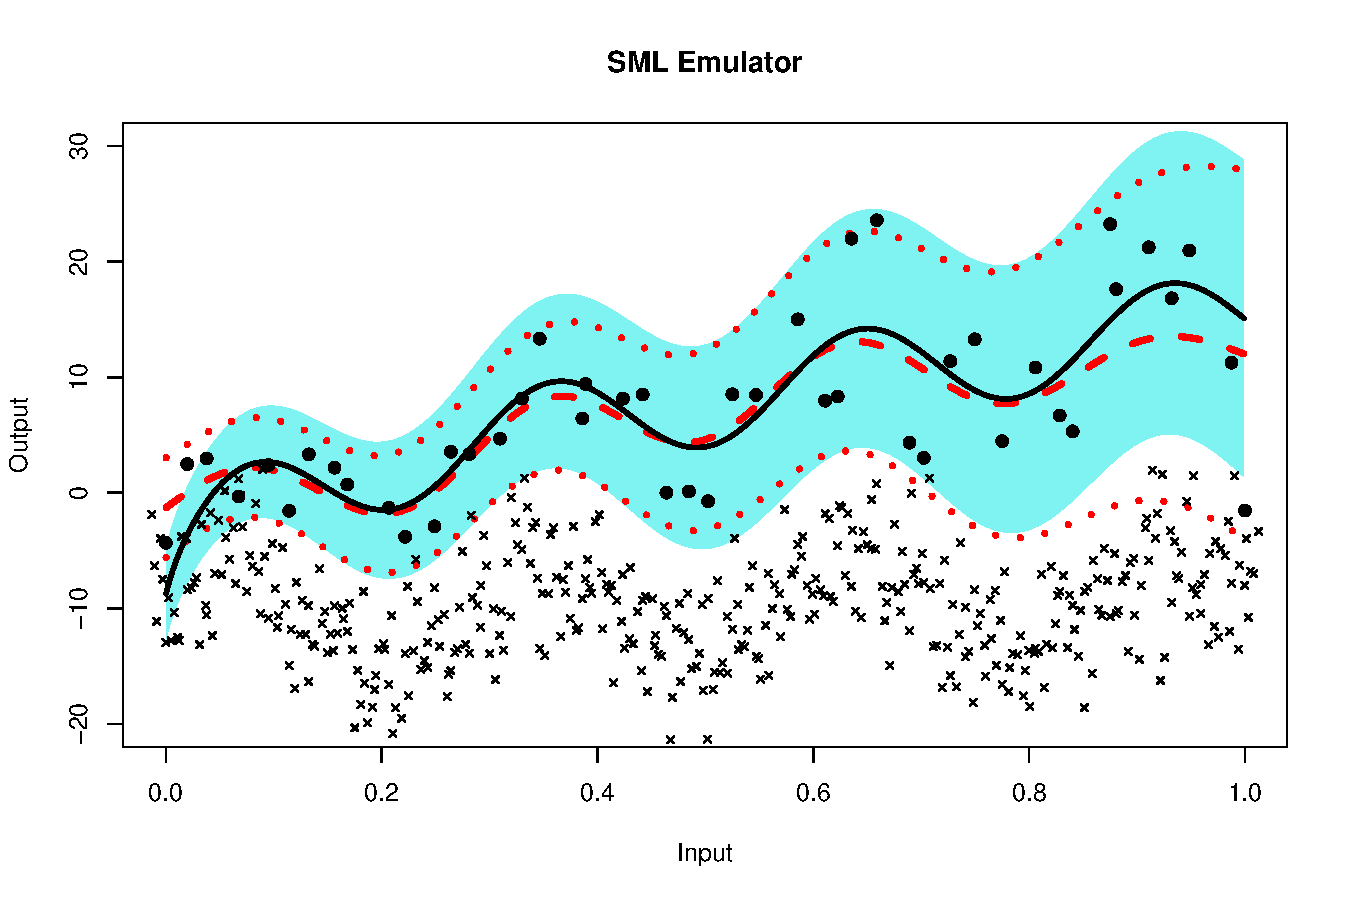
\includegraphics[width=0.75\textwidth]{sml-het-fig2/toy-sml.pdf}
	\caption{A SML emulator for $y(\cdot)$. Expensive runs are black points and cheap runs are black crosses (which are offset by $-10$ to aid visualisation). The true simulator is represented by the black line (mean function) and blue band ($\pm 1.96$ standard deviations). The emulator is represented by the red dashed line (emulator mean) and red dotted lines ($\pm 1.96$ emulator standard deviations).\label{Fig:comparison}}
\end{figure}

\section{Fitting HetGPs and SML Emulators to Athena}
As we discussed in the first chapter of this thesis, one task a subjective Bayesian may want to perform is a probabilistic sensitivity analysis (PSA) to better plan an elicitation exercise. Since Athena is stochastic, we want to understand
\begin{itemize}
	\item[(i)] which parameters influence the mean response
	\item[(ii)] which parameters influence the stochasticity.
\end{itemize}
To do such a task, with an expensive simulator such as Athena, we will first want to fit an appropriate emulator. HetGPs provide what we need here as they provide flexible estimates of both $\E\{y(\bx)\}$ and $\var\{y(\bx)\}$. The main output of Athena is availability, $A(\bx) \in (0,1)$. Since $A(\bx) \in (0,1)$ we will construct emulators for $y(\bx) = \probit (\bx) = \Phi^{-1}(\bx) \in \R$.  We will compare two approaches to fitting a HetGP to Athena.

Firstly, we will fit the emulator via MAP approach (which can also be thought as a penalised log-likelihood approach). This is partly to provide improved estimates of lengthscales as they can have a very flat likelihood. The second approach will be an Empirical Bayes (EB) approach; we will integrate out any $\beta$ terms in the emulator and find MAP estimates of aspects of the covariance functions. Here we \textit{will not} consider a full-Bayes approach (implemented via MCMC). This is because a full-Bayes approach is incredibly computationally costly due to (a) poor mixing in latent variable models and (b) multiple matrix inversions being required for each iteration of the MCMC scheme \citep{Kersting2007}.
\begin{comment}
\section{MAP Approach}

The MAP approach estimates $\Theta$ by
\begin{equation}
	\widehat{\Theta}  = \argmax_{\Theta} \pi(\Theta \mid \mathcal{D}).
\end{equation}
From a practical perspective, this estimation is performed via \verb|stan| via the \verb|Rstan| interface \citep{stan}.

The posterior distribution of $\log \lambda^2(\bx) \mid \Theta, \log \lambda^2(X)$ is straightforward to compute given estimated values of $\log \lambda^2(X)$. Note that in the MAP approach, we can treat the latent $\log \lambda^2(X)$ as unknown parameters. Thus the \verb|stan| programs used to estimate $\Theta$ also return estimates of $\log \lambda^2(X)$.

Prediction of simulator outputs at inputs $X^*$ first requires the predictive distribution of $\log \lambda^2 (X^*)$.
\begin{equation}
\log \lambda^2(X^*) | \log \lambda^2(X), \mathcal{D}, \Theta \sim \mathcal{N} \left\{ m_V^*(X^*), C_V^*(X^*, X^*) + \lambda_{V}^2 \right\}.
\end{equation}
where the posterior moments are found via the conditional normal equations,
\begin{align}
m^*_V(X^*) & = m_V(X^*) + C_V(X^*, X)
\left[C_V(X, X) + \lambda_{V}^2 I_n \right]^{-1}\left(\log \lambda^2(X) -  m_V(X) \right) \\
C_V^*(X^*, X^*) & = C_V(X^*, X^*) - C_V(X^*, X) \left[C_V(X, X) + \lambda_{V}^2 I_n \right]^{-1}C_V(X, X^*)
\end{align}
and $I_n$ is the $n \times n$ identity matrix.
Then conditional on the data, and hyperparameters, the posterior predictive distribution of the simulator at inputs $X^{*}$ is

\begin{equation}
y(\bx^*) | \Theta, \mathcal{D} \sim \mathcal{N} \left\{ m^*(X*) , C^* (X^*, X^*) + \lambda^{2*} (X^*) \right\}.
\end{equation}

Here, $\lambda^{* 2} (X^*) = \exp\{ m_V ^* (X^*) \}$ and $m^*(X^*)$, $C^* (X^*, X^*)$ are also found by the conditional normal equations:

\begin{align}
m^*(X^*) & = m(X^*) + C(X^*, X) \left[ C(X,X) + \lambda^{2 *} (X) I\right]^{-1}\left( \bm{y} - m(\bx) \right)  \\
C^*(X^*, X^*) & = C(X^*, X^*) -  C(X^*, X) \left[ C(X,X) + \lambda^{2 *} (X) I \right] ^{-1} C(X, X^*) \nonumber
\end{align}

where $\bm{y} = (y_1, \ldots, y_n)$.
\end{comment}
\subsection{Emulator construction}
\label{sec:em-con}

We construct emulators over a $9$ dimensional input space.  We vary each input over the range $[0.1, 5]$ (years). The Athena simulator is flexible enough to specify unique parameters for every subassembly in every turbine. We give the same parameter values to each subassembly of a given type and allow different types of subassembly to have different parameters. For example, all gearboxes could have a time to degradation of $1$ year whereas all generators could have a time to degradation of $3.2$ years.

Design points are chosen via the structure described in \Cref{Sec:design}. To construct the HetGP emulator we ran the Athena simulator at $100$ design points. The cheap runs of the simulator were fast enough that we could trade just $5$ expensive design points for $295$ cheap runs. We used basis functions $h(\bx) = (1, \log(\bx))$ for the mean functions of the mean response. We arrived at this selection to reflect a prior belief that the mean availability would flatten off at larger values of $x_i$. The covariance function assumes standardised inputs, $x_i^*$. Standardisation is achieved by subtracting the sample means and then dividing by the sample standard deviations (of the expensive training data). The latent variance GP has mean function $m_V(\bx) = (1, \bx^*)\bm{\beta}_V$ and again, the covariance function assumes standardised inputs.
\begin{figure}
	\centering
	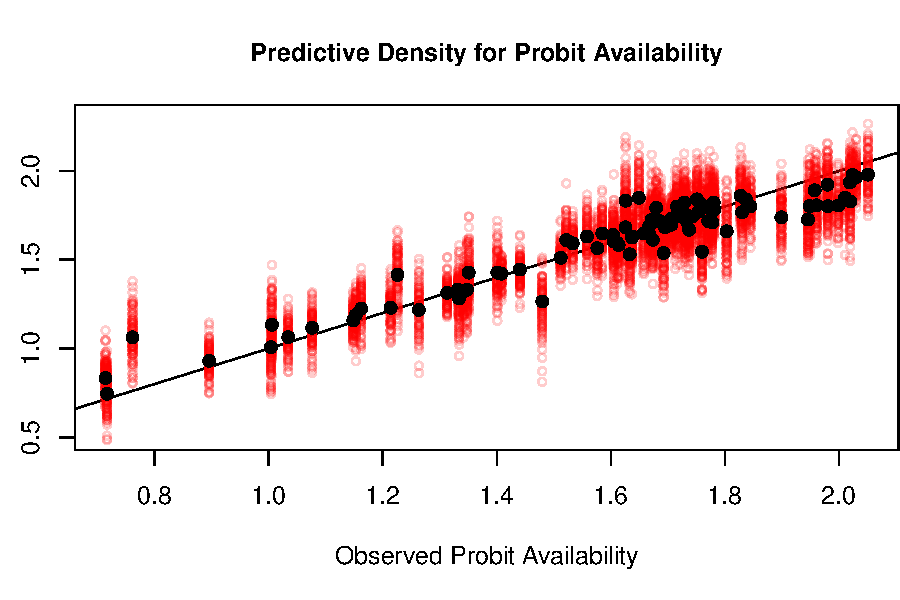
\includegraphics[width=0.7\textwidth]{sml-het-fig2/obs-pred-new.pdf}
\caption{Observed probit availability (training data) plotted against emulator mean predictions (black dots) and $100$ realisations from the emulator at each point (translucent red circles).\label{Fig:within-sample}}
\end{figure}
\Cref{Fig:within-sample} shows the emulator predictions of the training data (probit scale) with realisations from $\mathcal{N}\{m^{*}(\bx), v^{*}(\bx)\}$ around each prediction. Large deviations from the unit diagonal are typically accompanied by a more diffuse predictive distribution; the emulator is giving larger variance to the points which are far away from the mean. We also see that the observed probit availabilities are mostly in the region of $0.5$ -- $2$ (availabilities in the region of around $0.76$ -- $0.98$). The full range of observed availabilities is $(0.762, 0.980)$; the vast majority of realisations from the emulator agree with this range.

\subsection{Emulator performance comparison}

To judge relative performance of each emulator we use the performance metrics outlines in the previous chapter; RMSE  and Score (Equations \ref{Eq:rmse} and \ref{Eq:scoring-rule}). Using $100$ independently generated validation data points, the RMSE (on the probit scale) for HetGP was $0.181$, whereas SML achieved an RMSE of $0.156$. The score for HetGP was $238$ and for SML the score was $254$ (probit scale). Since we transformed the availability to construct emulators on an unbounded space, we should also check how predictions perform on the $[0,1]$ scale. Using an inverse-probit transformation on the mean function provides a sensible point estimate of availability. Comparing the MSE on the original scale  we observe an RMSE of $0.0272$ for HetGP, and under SML this is reduced to $0.0198$. Hence, SML achieves better RMSE and score here than HetGP for the Athena model, suggesting it is a better emulator. Further, our MAP estimate of $\rho$ is $\hat{\rho} = 0.51$. This suggests a moderate correlation between the two versions of Athena. The additional information extracted from cheap simulations has improved our emulation with little computational cost. It took $5.7$ seconds to fit HetGP and $29.6$ seconds to fit SML on a laptop with $4 \times 2.40\,\text{GHz}$ processors and $8\,\text{GB}$ RAM. Although SML took more time to fit, in real terms this is about $30$ seconds of computation time -- less than a single  expensive run of Athena. Both timings are for a total of $3$ fits of the emulator. We performed $3$ fits to prevent choosing a local mode as the MAP estimate.%KJW: a 'picture' of the emulator?

\subsection{Emulator validation}

To validate the emulators, we will implement some graphical diagnostics proposed by \citet{Bastos09}. Since we model the (transformed) simulator outputs by a Gaussian process, the Cholesky errors (CEs) should form a random sample from a $\mathcal{N}(0, 1)$ distribution (approximately). If the posterior mean and variance are well suited to the simulator, the validation data should lie in a horizontal band, centred at $0$, with approximately $95\%$ of points in the interval $(-1.96, 1.96)$. We also compare empirical quantiles of the CEs against theoretical quantiles -- we do this via coverage plots which compare the proportion of CEs in the $100(1-\alpha)\%$ prediction interval against the expected proportion.
\begin{figure}[!ht]
    \centering
       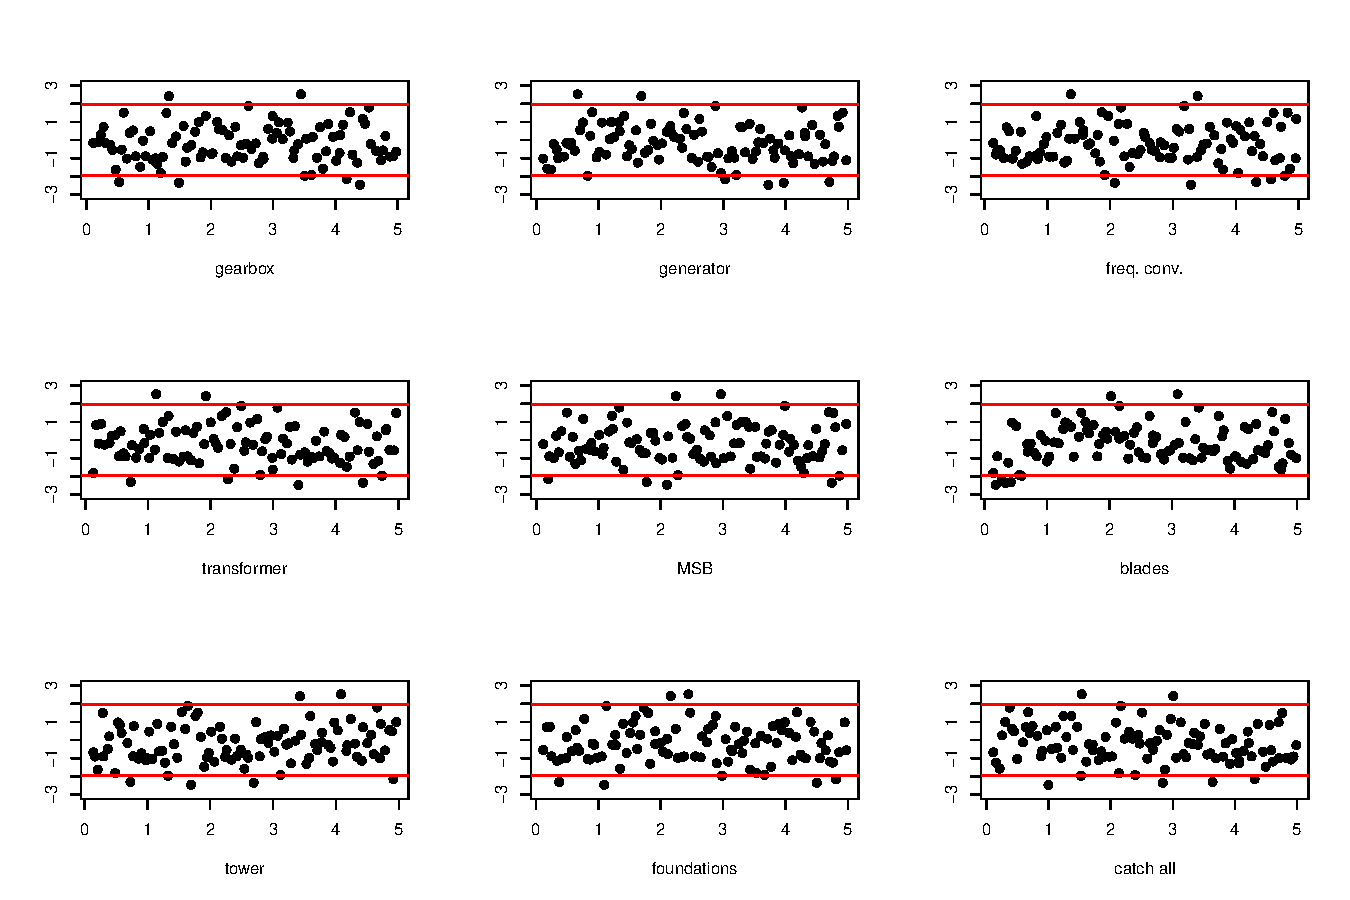
\includegraphics[width = 0.8\textwidth]{sml-het-fig2/het-resids-new3.pdf}
       \caption{Cholesky errors for HetGP, based on $100$ ``unseen'' validation points. Orange lines are at $\pm 1.96$.\label{Fig:het-resids}}
\end{figure}
\begin{figure}[!ht]
    \centering
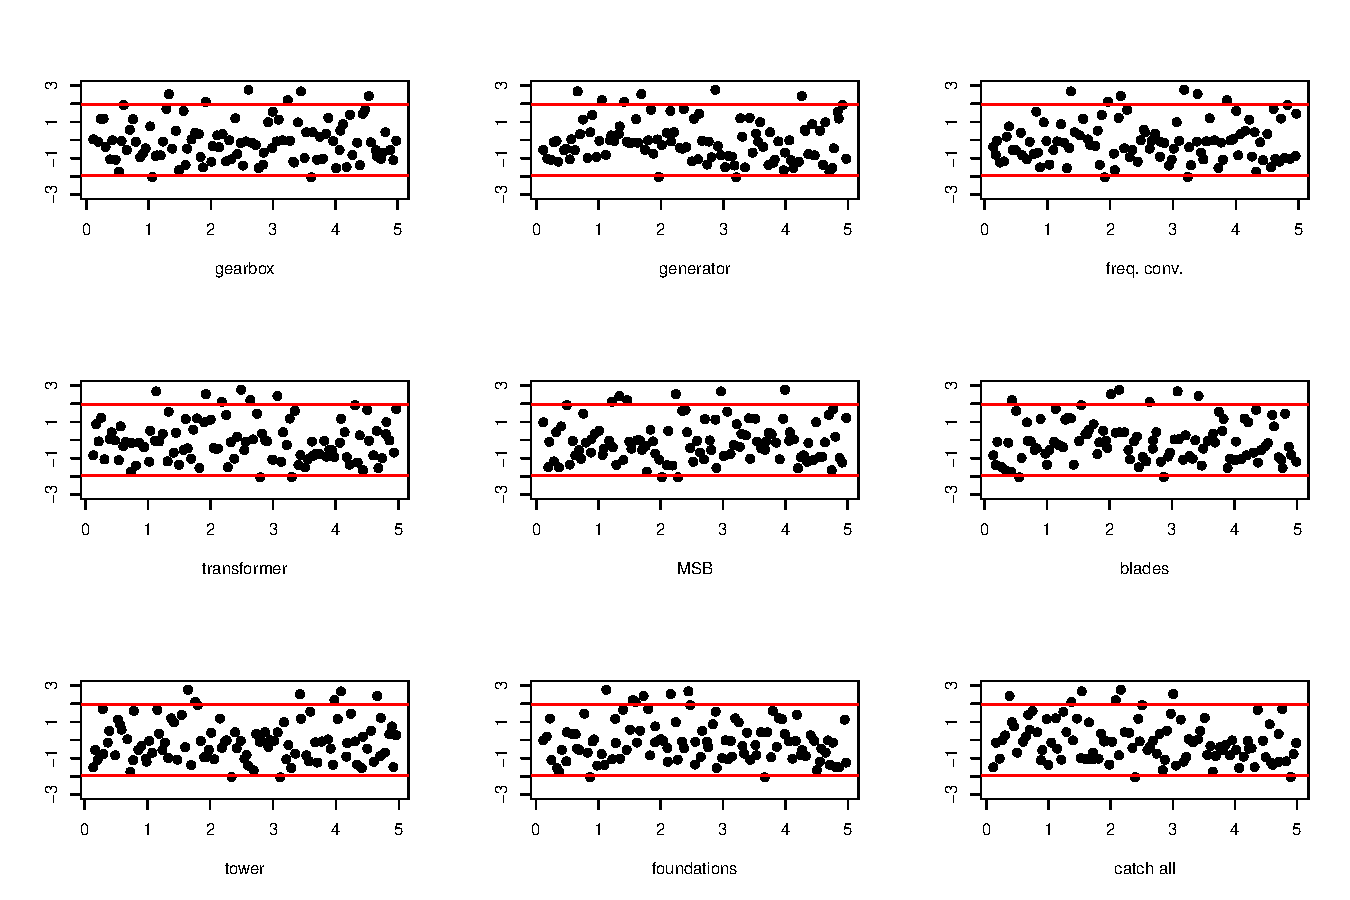
\includegraphics[width = 0.8\textwidth]{sml-het-fig2/sml-resids-new3.pdf}
\caption{Cholesky errors for SML emulation, based on $100$ ``unseen'' validation points. Orange lines are at $\pm 1.96$.\label{Fig:sml-resids}}
\end{figure}
\begin{figure}[!ht]
    \centering
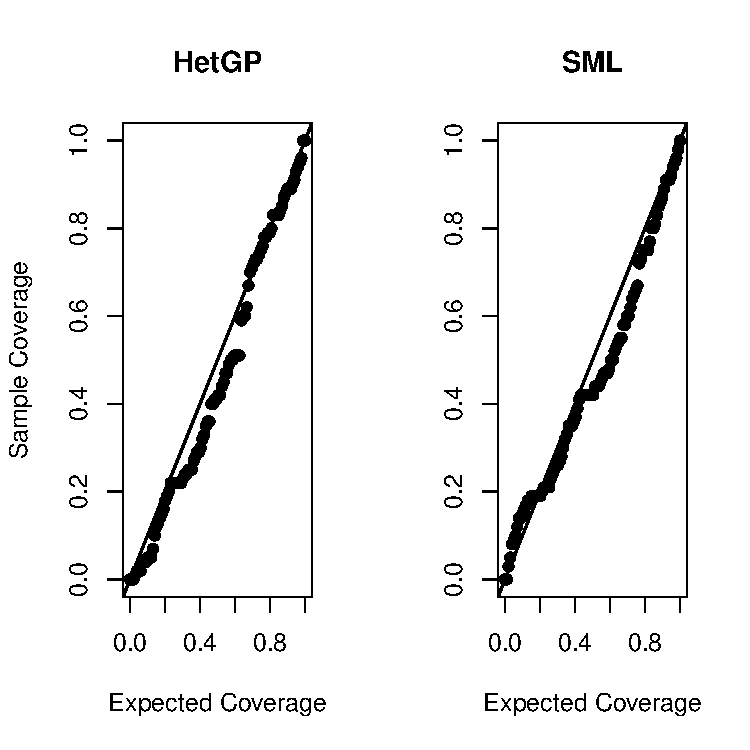
\includegraphics[width = 0.7\textwidth]{sml-het-fig2/coverage-new3.pdf}
    \caption{Out of sample coverage plots (black dots), using the Cholesky errors of the ``unseen'' validation data. Black lines represent the unit diagonal. \label{Fig:coverage}}
\end{figure}
In Figure~\ref{Fig:het-resids} the CEs for HetGP have a distinct pattern when plotted against $x_6$, whereas for SML in Figure~\ref{Fig:sml-resids} the points appear to be closer to a random $\mathcal{N}(0,1)$ sample.  The coverage plots in Figure~\ref{Fig:coverage} suggest that for both emulators the coverage is reasonably well calibrated.

\section{MAP Approach}

This chapter so far has taken a Bayesian approach to HetGP and SML. Although the approach is not fully Bayesian, it takes into account some parameter uncertainty without the crippling computational nightmares of MCMC and, at least in the illustrated Athena example, the Bayesian SML emulator provides a fairly accurate and efficient surrogate for the Athena simulator.

However, the majority of the literature uses a MAP/MLE approach to estimate GP hyperparameters and for prediction of simulator output \citep{Binois2018, Baker2020a, Baker2020c, Zhang2020, Baker2022}. Since this is a mathematically simpler approach, it would be worth investigating whether using the MAP estimate offers improved emulator accuracy and/or improves the computational properties of the emulator.


\subsection{Map-HetGP Prediction}

With the MAP approach, \emph{all} parameters are estimated by their posterior mode. Therefore we will re-define $\Theta := \{\Theta, \beta, \beta_V \}$. Given $\{\mathcal{D}, \Theta \}$, prediction follows in a similar way to the Bayesian version.

Like with the Bayesian version, we first predict $\log \lambda^2 (X^*)$. The predictive distribution of $\log \lambda^2 (X^*) \mid \Theta, \mathcal{D}$ is given by
\begin{equation}
	\log \lambda^2 (X^*) \mid \Theta, \log \lambda^2(X), \mathcal{D} \sim \mathcal{N} \{ m_V^*(X^*), v_V^*(X^*) \}
\end{equation}
where the posterior moments are
\begin{align}
	m_V^*(X^*) &= H_V^* \hat{\beta}_V + C_V(X^*, X)\left\{ C_V(X, X) + \lambda^2_V I \right\}^{-1} ( \log \lambda^2 (X) - H_V \hat{\beta}_V ) \\
	v_V^*(X^*) &= C_V(X^*, X^*) - C_V(X^*, X)\left\{ C_V(X, X) + \lambda^2_V I \right\}^{-1} C_V(X, X^*) + \lambda^2_V I.
\end{align}
As with the Bayesian version, there are three plug-in estimates of $\lambda^2(X^*)$ that can be used. For simplicity, we use $\lambda^2(X^*) = \exp\{ m_V^*(X^*) \}$. With this estimate, we can then write the predictive distribution of $y(X^*)$ as
\begin{equation}
	y(X^*) \mid \Theta,\lambda^2(X), \mathcal{D} \sim \mathcal{N} \{ m^*(X^*), v^*(X^*) \}
\end{equation}
where the posterior moments are
\begin{align}
	m^*(X^*) &= H^* \hat{\beta} + C(X^*, X)\left\{ C(X, X) + \lambda^2(X) I \right\}^{-1} ( y(X) - H \hat{\beta} ) \\
	v^*(X^*) &= C(X^*, X^*) - C(X^*, X)\left\{ C_V(X, X) + \lambda^2 I \right\}^{-1} C(X, X^*) + \lambda^2(X^*) I.
\end{align}
Note that these predictive equations are essentially the same as the Bayesian versions with $B = 0$, $B_V = 0$, $\bm{b} = \hat{\beta}$ and $\bm{b}_V = \hat{\beta}_V$
\subsection{MAP-SML Prediction}

Much like MAP-HetGP, MAP-SML prediction is obtained by taking the Bayesian versions of the predictive equations but setting prior variance matrices to $0$ and the regression coefficients to their MAP estimates. The design is independent of the statistical paradigm thus we use exactly the same design as above. Since the predictive equations are a direct consequence of the multivariate Normal equations, we present them without proof.

As usual, we start with prediction of the log variance.  $\log \lambda^2_E(X^*) \mid \Theta$ is multivariate normal with the following first two moments
\begin{align}
	m_V^*(X^*) &= H_V^* \hat{\beta}_V + C_V(X^*, X) \left\{C_V(X, X) + \lambda_V^2 I \right\}^{-1} (\log \lambda^2 (X) - H_V\hat{\beta}_V) \\
	v_V^*(X^*) &= C_V(X^*, X^*) - C_V(X^*, X) \left\{C_V(X, X) + \lambda_V^2 I \right\}^{-1} C_V(X, X^*) + \lambda^2_V I/.
\end{align}
The quantity of interest, $y^E(X^*)$, is also multivariate Normal, conditional on $\Theta, \lambda^2_E(X)$ and $\lambda_E^2(X^*)$ with mean and variance
\begin{align}
	m_E^*(X^*) &= H_V^* \hat{\beta}_V +C_0(X^*) \var(\bm{Y} \mid \Theta)^{-1} (\log \lambda^2 (X) - H_V\hat{\beta}_V) \\
	v_E^*(X^*) &= C_0(X^*, X^*) - C_0(X^*, X) \left\{C_0(X, X) + \lambda_V^2 I \right\}^{-1} C_0(X, X^*) + \lambda^2_E(X^*)I
\end{align}
where $C_0(X', X) = \cov(y^E(X'), y^E(X)) = \rho^2C_C(X', X) + C_E(X, X')$.

\subsection{Performance of MAP estimation}

The advantage of MAP estimation is that it is simpler and, if the user desired, a suitability diffuse prior would return an approximate maximum likelihood estimate. Ultimately, we want to know which performs best. Using the same priors as the Bayesian version to produce a MAP estimate, we refit the emulators and re-compute out of sample performance metrics using exactly the same validation data as before.

The performance of the MAP-based, and Bayesian, emulators are summarised in \Cref{Tab:all-performance}. All metrics in this table indicate that the Bayesian SML emulator is the best in terms of mimicking the Athena simulator. The Bayesian SML emulator does not have the fastest estimation routine, the Bayesian HetGP is fastest. However, this computation time is trivial relative to the computational cost of uncertainty analysis in a computationally expensive simulator such as Athena. The MAP-SML emulator has comparable performance to the Bayesian HetGP emulator in terms of RMSE (probit scale) and score, but the RMSE $(0,1)$ scale. although the MAP-SML emulator took a relatively long time to fit and will be slower to implement due to the larger design matrix. The MAP-HetGP offers a marginally better RMSE than its Bayesian equivalent, however the uncertainty quantification under the MAP approach is poor. The score is only $136$ (the Bayesian version had a score or $238$), this poor performance is exemplified by the C.E.s of the Map-HetGP which have a range of $(-3.85, 4.33)$. Overall, this stresses that incorporating parameter uncertainty into predictions, especially when the sample size is small, is a wise idea.

\begin{table}
	\centering
	\begin{tabular}{lrrrr}
		\toprule
		& \multicolumn{2}{c}{MAP} & \multicolumn{2}{c}{Bayes}\\
		Metric & HetGP & SML & HetGP & SML \\ \cmidrule{1-5}
		Time to fit emulator/seconds &$37$&$307$&$6$&$30$\\
		RMSE (probit scale)& $0.179$ & $0.171$&$0.181$&$0.156$\\
		RMSE ($(0,1)$ scale) &$0.0248$&$0.0231$&$0.0272$&$0.0198$\\
		Score &$136$&$248$&$238$&$254$\\\bottomrule
	\end{tabular}
	\caption{Performance summaries for the emulators based on both the MAP and Bayesian versions of the HetGP and SML emulators. Time here denotes the time take for a total of 3 runs of each estimation routine. RMSE and score are correct to $3$ s.f., time is correct to the nearest second.}
	\label{Tab:all-performance}
\end{table}
\section{Summary}
We have reviewed some approaches to emulating stochastic computer models which exhibit input dependent noise. We began with approaches which emulate the mean and variance as separate components and then moved over to a single, but more complex, emulator approach. We illustrated that HetGPs can suffer from poor predictive performance in the low-data regime, which is unfortunate since emulators typically constructed when data are expensive to obtain. We offered a solution to this by adapting the autoregressive model from \citet{Kennedy2000}

We have introduced a stochastic multilevel emulator, which adopted elements of (i) the autoregressive structure from \cite{Kennedy2000} to construct a more accurate mean function and (ii) the latent variance structure of HetGP \citep{Goldberg1998, Binois2018} to account for the heteroscedastic nature of the Athena simulator. This structure allowed us to link together two versions of the Athena simulator to construct an emulator with improved accuracy in terms of RMSE and also in terms of score. The easy to generate training data allowed us to build an adequate emulator without relying on a large computational budget to generate training data.

It would be interesting to see, from a methodological point of view, how the SML emulator could be improved. One idea would be to implement a sequential design rule similar to that of \citet{Gratiet2015}, that is, minimising some design criterion such as integrated mean squared prediction error. Another idea would be to use a preliminary round of simulations to see where cheap simulations might be most beneficial. For example, it may be advantageous to place more cheap points where the two levels agree most and then retain the expensive simulation budget for areas where the two levels disagree. It would also be interesting to see if replicates could improve this type of emulator in the same way that replicates benefit HetGP. Replication could be especially beneficial in the cheap simulator; this would help to reduce the size of computational overheads of a large design matrix since inference is $\mathcal{O}(N^3)$ for HetGP and $\mathcal{O}\left((N_C+N_E)^3\right)$ for SML, however \cref{Tab:all-performance} showed that the raw computation times for the Athena simulator were not particularly large. Prediction is $\mathcal{O}\left(N^2\right)$ for HetGP and $\mathcal{O}\left((N_C+N_E)^2\right)$ for SML. Another possibility would be to link the variance of the two simulators; we chose not to do this as it would involve linking two latent variance processes and would involve inversion of a large matrix, increasing the computational cost of inference and prediction.

An alternative approach to using cheap simulations to help build an accurate emulator based on cheap simulations is to use a large number of cheap simulations to construct an informative prior for $y^E(\cdot)$. This could be more computationally efficient than the SML emulator, but would likely require more human input. The informative prior would then be used as part of a HetGP emulator for $y^E(\cdot)$. \citet{Cumming2010} use a large number of runs from a cheap, deterministic simulator to build an informative prior for an expensive, deterministic simulator. Their idea could be adapted to the stochastic, heteroscedastic case in the following way: first use the two-emulator approach of \citet{Henderson09} to obtain an emulator for $y^C(\cdot)$. Next use the MCMC samples obtained from $\pi(\Theta_C \mid \mathcal{D})$ where $\Theta_C$ are the hyperparameters of the GP fitted to $y^C(\cdot)$ to obtain $\pi(\Theta_E)$, the prior for the hyperparameters of $y^E (\cdot)$. Finally, use $\pi(\Theta_E)$ to fit an emulator to $y^E (\cdot)$. We provide no specific details of how to perform such an elicitation, but when constructing $\pi(\Theta_E)$ the analyst should consider how they think the versions of the simulator differ, rather than just setting $\pi(\Theta_E) = \pi(\Theta_C \mid \mathcal{D})$. \citet{Cumming2010} give advice on how to do this within a Bayes Linear framework; much of their approach could be applied to a Full Bayesian (or our partially Bayesian) approach.

\end{chapter}
